\documentclass[a4paper,14pt]{extarticle}

\usepackage[T2A]{fontenc}
\usepackage[utf8]{inputenc}
\usepackage[russian]{babel}
\usepackage{geometry}
\usepackage{setspace}
\usepackage{indentfirst}
\usepackage{array}
\usepackage{booktabs}
\usepackage{listings}
\usepackage{xcolor}
\usepackage{graphicx}
\usepackage{caption}

\geometry{
    left=30mm,
    right=15mm,
    top=20mm,
    bottom=20mm
}

\onehalfspacing
\setlength{\parindent}{1.25cm}
\setlength{\parskip}{0pt}
\setlength{\emergencystretch}{3em}

\lstdefinestyle{codestyle}{
    basicstyle=\ttfamily\small,
    frame=single,
    breaklines=true,
    showstringspaces=false
}

\begin{document}

\begin{titlepage}
\begin{center}
\textbf{МОСКОВСКИЙ АВИАЦИОННЫЙ ИНСТИТУТ}\\
\textbf{(НАЦИОНАЛЬНЫЙ ИССЛЕДОВАТЕЛЬСКИЙ УНИВЕРСИТЕТ)}\\
Институт №8 «Компьютерные науки и прикладная математика»
\end{center}

\vspace{3.5cm}
\begin{center}
\textbf{\Large Курсовой проект}\\
\vspace{0.3cm}
по курсу «Технологии параллельного программирования»\\
\vspace{0.8cm}
\textbf{Обратная трассировка лучей (Ray Tracing) на GPU}
\end{center}

\vspace{4cm}
\begin{flushright}
Выполнил: Ахметшин Б.Р.\\
Группа: М8О-403Б-22\\
Преподаватели: А.Ю. Морозов,\\
\hspace*{3.6cm} Е.Е. Заяц
\end{flushright}

\vfill
\begin{center}
Москва, 2026
\end{center}
\end{titlepage}

\section*{Условие}
Цель работы: использование GPU для ускорения визуализации сцены методом
обратной трассировки лучей, построение анимации и сравнение производительности
GPU и CPU реализаций.

По условию требуется сцена с тремя платоновыми телами, источниками света,
анимированной камерой, сглаживанием (SSAA), а также вывод статистики
по каждому кадру.

В выполненной работе реализован вариант с телами:
\textbf{тетраэдр, гексаэдр, икосаэдр} (вариант 3).

\section*{Программное и аппаратное обеспечение}
\textbf{GPU}

\begin{tabular}{>{\raggedright\arraybackslash}p{0.50\textwidth}>{\raggedright\arraybackslash}p{0.34\textwidth}}
Имя & NVIDIA Tesla T4 \\
Compute Capability & 7.5 \\
Объем глобальной памяти & 15637086208 \\
Разделяемая память на блок & 49152 \\
Константная память & 65536 \\
Регистров на блок & 65536 \\
Макс. потоков на блок & (1024, 1024, 64) \\
Макс. размер сетки & (2147483647, 65535, 65535) \\
Количество мультипроцессоров & 40 \\
\end{tabular}

\vspace{0.4cm}
\textbf{CPU}

\begin{tabular}{>{\raggedright\arraybackslash}p{0.50\textwidth}>{\raggedright\arraybackslash}p{0.34\textwidth}}
Архитектура & x86\_64 \\
CPU op-mode(s) & 32-bit, 64-bit \\
Address sizes & 48 bits physical, 48 bits virtual \\
Порядок байт & Little Endian \\
CPU(s) & 12 \\
Имя модели & AMD Ryzen 5 7600 6-Core Processor \\
Ядер / потоков & 6 / 12 \\
\end{tabular}

\vspace{0.4cm}
\textbf{RAM}\\
64 GB

\vspace{0.2cm}
\textbf{ОС}\\
Ubuntu 24.04.4 LTS

\vspace{0.2cm}
\textbf{Компиляторы}\\
g++, nvcc

\section*{Метод решения}
В проекте реализован трассировщик первичных лучей для полигональной сцены.

Основные этапы:
\begin{enumerate}
    \item Для каждого пикселя строится луч из позиции камеры через плоскость
    изображения.
    \item Для каждого луча ищется ближайшее пересечение с треугольниками сцены
    (алгоритм Möller--Trumbore).
    \item Если пересечение найдено, цвет вычисляется по локальной модели
    освещения (ambient + diffuse/Lambert).
    \item Для теней запускается теневой луч к источнику света
    (простая hard-shadow модель).
    \item Для сглаживания используется SSAA: на пиксель трассируется
    \(ssaaSqrt^2\) лучей с усреднением результата.
\end{enumerate}

Положение камеры и точки наблюдения меняется по кадрам по параметрическим
законам в цилиндрических координатах, что обеспечивает облет сцены.

\textbf{Текущие ограничения реализации:}
без рекурсии, без отражений и прозрачности, без текстур пола,
используется один источник света из входной конфигурации.

\section*{Описание программы}
\textbf{Структура проекта}
\begin{itemize}
    \item \texttt{src/domain/*} --- геометрия, математика, генерация сеток
    платоновых тел.
    \item \texttt{src/application/*} --- конфигурация, построение сцены,
    расчет положения камеры по кадрам, оркестрация рендера.
    \item \texttt{src/adapters/cpu/cpu\_renderer.cpp} --- CPU реализация рендера.
    \item \texttt{src/adapters/gpu/cuda\_renderer.cu} --- CUDA реализация рендера.
    \item \texttt{src/adapters/file/ppm\_writer.cpp} --- запись кадров в PPM (P6).
    \item \texttt{src/adapters/cli/main.cpp} --- разбор ключей запуска и старт приложения.
\end{itemize}

\textbf{Ключи запуска}
\begin{itemize}
    \item \texttt{--cpu} --- рендер только на CPU;
    \item \texttt{--gpu} --- рендер на GPU (режим по умолчанию);
    \item \texttt{--default} --- печать дефолтной конфигурации в stdout и выход.
\end{itemize}

\textbf{Формат статистики во время работы}
\begin{lstlisting}[style=codestyle]
{frame_idx}\t{frame_time_ms}\t{total_rays}
\end{lstlisting}

\textbf{Пример входной конфигурации}
(использована в тестах, формат соответствует парсеру проекта):
\begin{lstlisting}[style=codestyle]
16
out/frame_%d.ppm
640 480 100
7.0 3.0 0.0
2.0 1.0
2.0 6.0 1.0
0.0 0.0
2.0 0.0 0.0
0.5 0.1
1.0 4.0 1.0
0.0 0.0
-2.0 -0.6 0.8
1.0 0.2 0.2
1.0 0.0 0.0 0
0.2 1.1 1.0
0.1 0.9 0.2
1.2 0.0 0.0 0
2.0 -0.8 1.1
0.2 0.5 1.0
1.3 0.0 0.0 0
-6.0 -6.0 -1.0
-6.0 6.0 -1.0
6.0 6.0 -1.0
6.0 -6.0 -1.0
-
0.8 0.8 0.85 0.0
1
-2.0 -1.0 7.0
1.0 1.0 1.0
1 1
\end{lstlisting}

\section*{Исследовательская часть и результаты}
Проведено сравнение производительности CPU и GPU на одинаковой сцене.
Измерялось время построения кадра (мс) и анализировалась стабильность времени
на последовательности кадров.

\textbf{Замеры времени (среднее по 16 кадрам):}
\begin{lstlisting}[basicstyle=\ttfamily\scriptsize,frame=single]
+----+----------+----------+-----------+-----------+
| No | res      | ssaaSqrt | CPU, ms   | GPU, ms   |
+----+----------+----------+-----------+-----------+
| 1  | 640x480  | 1        | 221.250   | 20.562    |
+----+----------+----------+-----------+-----------+
| 2  | 640x480  | 2        | 788.688   | 24.188    |
+----+----------+----------+-----------+-----------+
| 3  | 960x540  | 1        | 300.438   | 24.625    |
+----+----------+----------+-----------+-----------+
| 4  | 960x540  | 2        | 1358.188  | 23.938    |
+----+----------+----------+-----------+-----------+
| 5  | 1280x720 | 1        | 575.375   | 25.250    |
+----+----------+----------+-----------+-----------+
| 6  | 1280x720 | 2        | 2300.188  | 30.063    |
+----+----------+----------+-----------+-----------+
\end{lstlisting}

\textbf{Замечание по прогреву:}
первый кадр в GPU-режиме существенно медленнее (около 295--342 ms),
далее время стабилизируется на уровне 2--15 ms в зависимости от режима.

\textbf{Профилирование GPU (\texttt{nvprof}):}
\begin{lstlisting}[style=codestyle]
==3211== NVPROF is profiling process 3211, command: ./kp --gpu
==3211== Profiling application: ./kp --gpu
==3211== Profiling result:
            Type  Time(%)      Time     Calls       Avg       Min       Max  Name
 GPU activities:   64.79%  1.0605ms         1  1.0605ms  1.0605ms  1.0605ms  [CUDA memcpy DtoH]
                   35.14%  575.16us         1  575.16us  575.16us  575.16us  renderKernel(...)
                    0.08%  1.2480us         1  1.2480us  1.2480us  1.2480us  [CUDA memcpy HtoD]
\end{lstlisting}

\textbf{Анализ результатов:}
\begin{itemize}
    \item Во всех сравнениях GPU быстрее CPU по среднему времени кадра.
    По среднему времени (включая первый кадр) ускорение составляет примерно
    от 8x до 76x в зависимости от режима.
    \item По покадровым логам видно выраженный эффект прогрева GPU:
    первый кадр занимает сотни миллисекунд, а последующие кадры обычно
    2--10 ms. Если исключить первый кадр, ускорение GPU относительно CPU
    возрастает до десятков и сотен раз.
    \item Увеличение SSAA с 1 до 2 существенно повышает стоимость рендера
    (число лучей на пиксель возрастает в 4 раза), что подтверждается ростом
    времени и для CPU, и для GPU.
    \item Логи \texttt{nvprof} показывают, что в профилируемом прогоне заметную
    долю занимают копирования, особенно \texttt{DtoH} (64.79\%), тогда как
    вычислительный \texttt{renderKernel} занимает 35.14\%.
\end{itemize}

\textbf{Примеры кадров}
\newline
Собранная анимация: \texttt{out/perf\_640x480\_ssaa1\_cpu.gif}

\begin{figure}[ht]
\centering
\begin{minipage}{0.49\textwidth}
\centering
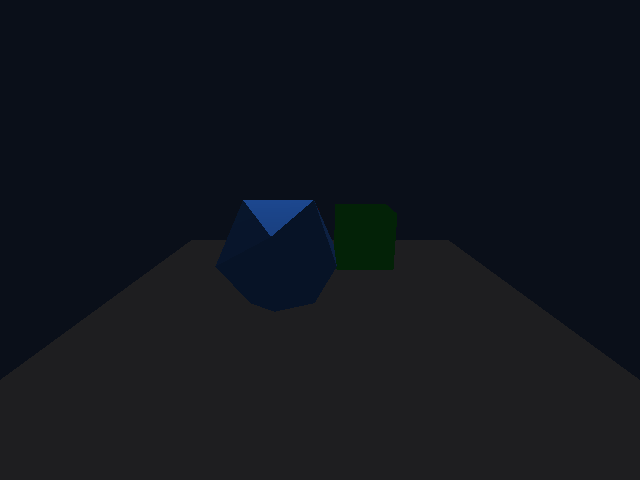
\includegraphics[width=\linewidth]{report_assets/frame_cpu_0000.png}
\caption*{Кадр 0}
\end{minipage}
\hfill
\begin{minipage}{0.49\textwidth}
\centering
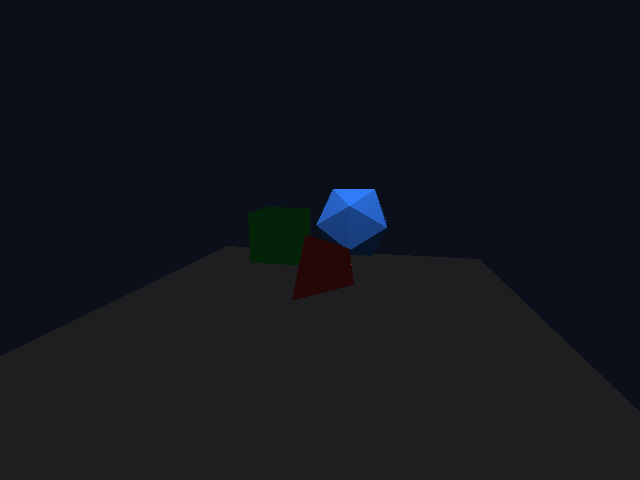
\includegraphics[width=\linewidth]{report_assets/frame_cpu_0008.png}
\caption*{Кадр 8}
\end{minipage}
\caption{Кадры сцены при разрешении 640x480, SSAA=1}
\end{figure}

\section*{Выводы}
В курсовом проекте реализован рендеринг трехмерной сцены методом обратной
трассировки лучей в двух режимах: CPU и GPU (CUDA). Реализация корректно
обрабатывает анимированную камеру, SSAA и выводит покадровую статистику.

Экспериментальные замеры подтверждают существенное ускорение GPU по
сравнению с CPU. При этом для GPU явно наблюдается большой накладной расход
первого кадра (инициализация контекста и выделение/копирование памяти), тогда как
последующие кадры рендерятся значительно быстрее.

Профилирование показало, что в текущей реализации заметная часть времени уходит
на копирование результата из памяти устройства на хост, а не только на сам kernel.
Это означает, что дальнейшие оптимизации целесообразно направлять на уменьшение
объемов/частоты обмена и переиспользование буферов между кадрами.

Архитектура проекта (domain / application / adapters / ports) обеспечивает хорошую
расширяемость для следующих этапов: добавление рекурсии, отражений,
прозрачности, текстур и более сложной модели освещения.

\end{document}
